\section{Revisión bibliográfica}

El problema de clasificación de un tipo concreto de comida no es un problema muy común y por lo tanto estudiado. Como hemos visto en clase de teoría, el auge de la visión por computador se ha dado en el comienzo de la década del 2010, hace apenas diez años, con la aparición de modelos basados en redes neuronales convolucionales a pesar de que el modelo teórico de neurona y red neuronal llevan más tiempo en el ámbito de la informática. Esto ha sido en parte gracias al aumento de la capacidad de cómputo de los procesadores (tanto CPUs como procesadores gráficos) actuales.

Por este motivo, como era de esperar, en estos últimos diez años el uso de redes neuronales convolucionales se ha centrado en mejorar sus resultados con distintas técnicas vistas en teoría, mejorar los tiempos de ejecución buscando algoritmos eficientes o simplemente aumentando la potencia de cómputo, y los problemas que se han tratado de resolver son problemas más generales y en el caso de tratar algún problema específico se trata de un problema de gran interes común.

Estos motivos han llevado a que actualmente no se encuentre una gran cantidad de lecturas sobre nuestro problema concreto y las pocas que encontramos se tratan en su mayoría de comida en general sin distinguir su orgigen concreto, además de que estos experimentos comienzan a ser publicados a partir del año 2018.


En este año encontramos un trabajo de tres investigadores de la Universidad de Indonesia sobre detección de comida tradicional de Betawi en imágenes\cite{betawiFood}. En este paper se intenta detectar este tipo de comida utilizando una red ya preentrenada con otro conjunto de datos, un problema muy similar al nuestro, donde se obtienen unos resultados aceptables con una precisión de entre el 70\% y el 80\% dependiendo de la complejidad de la red utilizada.

Este es uno de los artículos que hemos encontrado donde se comienza a trabajar el problema de detección de comida, ya que como vemos en el paper citado como trabajos relacionados e introducción podemos encontrar que este trabajo surgió de una red neuronal profunda que consiguió muy buenos resultados a la hora de clasificar vehículos usando transferencia de conocimiento de una red ya preentrenada, por lo que los investigadores se interesaron en esto debido al gran impacto que conlleva el sector culinario en su país de origen.

Con respecto a la metodología aplicada en el artículo, vemos como se centran en aplicar un ajuste fino y reentrenar únicamente las últimas capas de distintos modelos basados en ResNet y DenseNet de cara a reentrenar la parte de la red que aplica la clasificación como tal y no la extracción de características, evitando tener que reentrenar toda la red completa con el coste computacional que conlleva. Vemos como esto le da unos resultados bastante buenos, siendo el peor caso la red ResNet101 con un 70\% de precisión, y el mejor caso DenseNet169 con una precisión del 80\%.


Como conclusiones de este trabajo encontramos que, si se realiza de forma correcta, el realizar un ajuste fino de una red con el nuevo conjunto de imágenes a entrenar podemos obtener un buen resultado, por lo que será lo primero que intentaremos hacer en nuestro proyecto, y a partir de ahí decidir si es necesario modificar las distintas capas de la red (ya sea añadiendo o eliminando capas), de cara a buscar unos mejores resultados.


\vspace{5 mm}

El día 27 de Octubre de 2018 se presentó en una conferencia del \textbf{ICACSIS} un paper llamado \textit{Betawi Traditional Food Image Detection using
ResNet and DenseNet}. Este paper se centraba en usar diferentes arquitecturas de Deep-Learning para detectar imágenes de platos de la cocina tradicional Betawi, quedándose finalmente con el mejor modelo encontrado.

\vspace{3 mm}

En este paper se usaron 1400 imágenes repartidas en el conjunto de training y de test usando un K-fold con k = 5. El proceso de entrenamiento se realizó en cada caso dos veces usando 5 épocas la primera vez, y 10 épocas la segunda.

\vspace{3 mm}

El paper usa 2 arquitecturas de Deep-Learning diferentes, \textbf{ResNet(50,101,152)} y \textbf{DenseNet(121,161,169)}. La diferencia entre cada una de las versiones anteriores reside en el número de capas que se usan. Cuantas más capas se usen, más bajo el error de la función de pérdida.

\vspace{3 mm}

Para evaluar cada una de las arquitecturas se usa el \textbf{accuracy} como métrica y el \textbf{cross entropy loss} como función de pérdida. Para comparar cada una de las arquitecturas entre ellas se ha hecho un ranking de los valores de cada arquitectura normalizados. La tabla con el ranking mencionado es la siguiente:

\vspace{5 mm}

\begin{figure}[H]
  \centering
  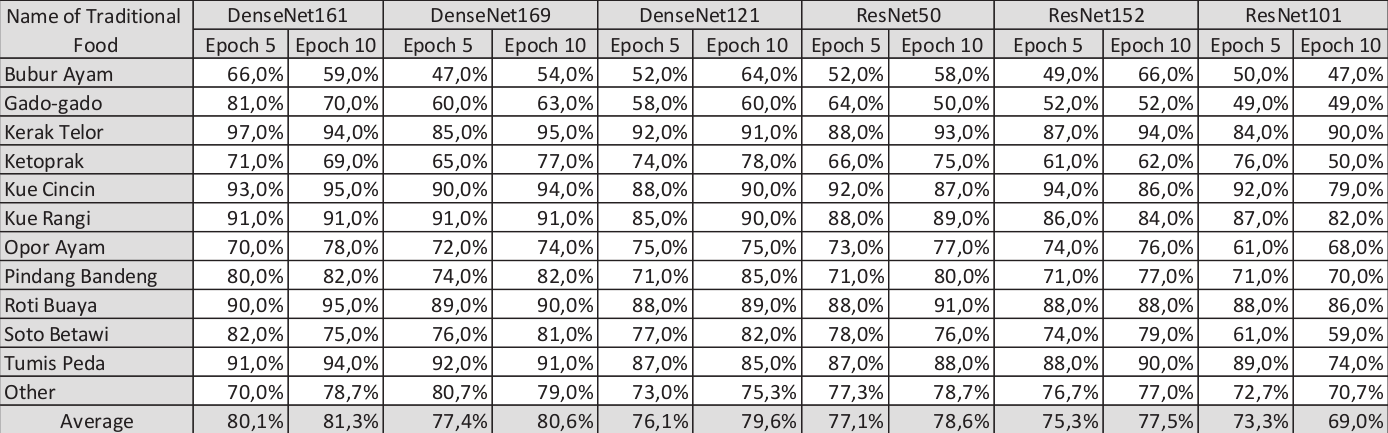
\includegraphics[width=1\linewidth]{Imagenes/tablapaper1.png}
  \caption{Accuracy de Testing}
  \label{fig:sub-first}
\end{figure}

\vspace{5 mm}

Al analizar la tabla, en el paper se llega a la conclusión de que una arquitectura será mejor u otra dependiendo de si se usa CPU o GPU en el proceso de entrenamiento. La arquitectura que mejor detecta los platos tradicionales Betawi es \textbf{DenseNet169} usando CPU y \textbf{ResNet50} usando GPU. Tendremos en cuenta estos resultados a la hora de implementar nuestro proyecto.

\newpage

Tan solo medio año despues dos investigadores de Google Research publicaron una publicación llamada \textit{EfficientNet: Rethinking Model Scaling for Convolutional Neural Networks}\cite{efficient}. Aunque esta publicación se centra en mejorar el escalado de redes neuronales convolucionales, una de las bases de datos utilizada será \textbf{Food101}, a pesar ser un problema más general que el nuestro, nos puede llegar a ser de gran utilidad debido a sus similitudes.

El principal objetivo de este trabajo se centra en explicar las diferencias entre los tipos de escalado de una red neuronal, así como buscar un equilibrio entre dichos escalados de cara a encontrar una red neuronal en la que se consigan buenos resultados, minimizando el número de parámetros de la red, y por lo tanto que el coste computacional sea menor.

Los tipos de escalado, como hemos visto, pueden ser en profundidad, en anchura, y en resolución de una misma capa.


\begin{figure}[H]
  \centering
  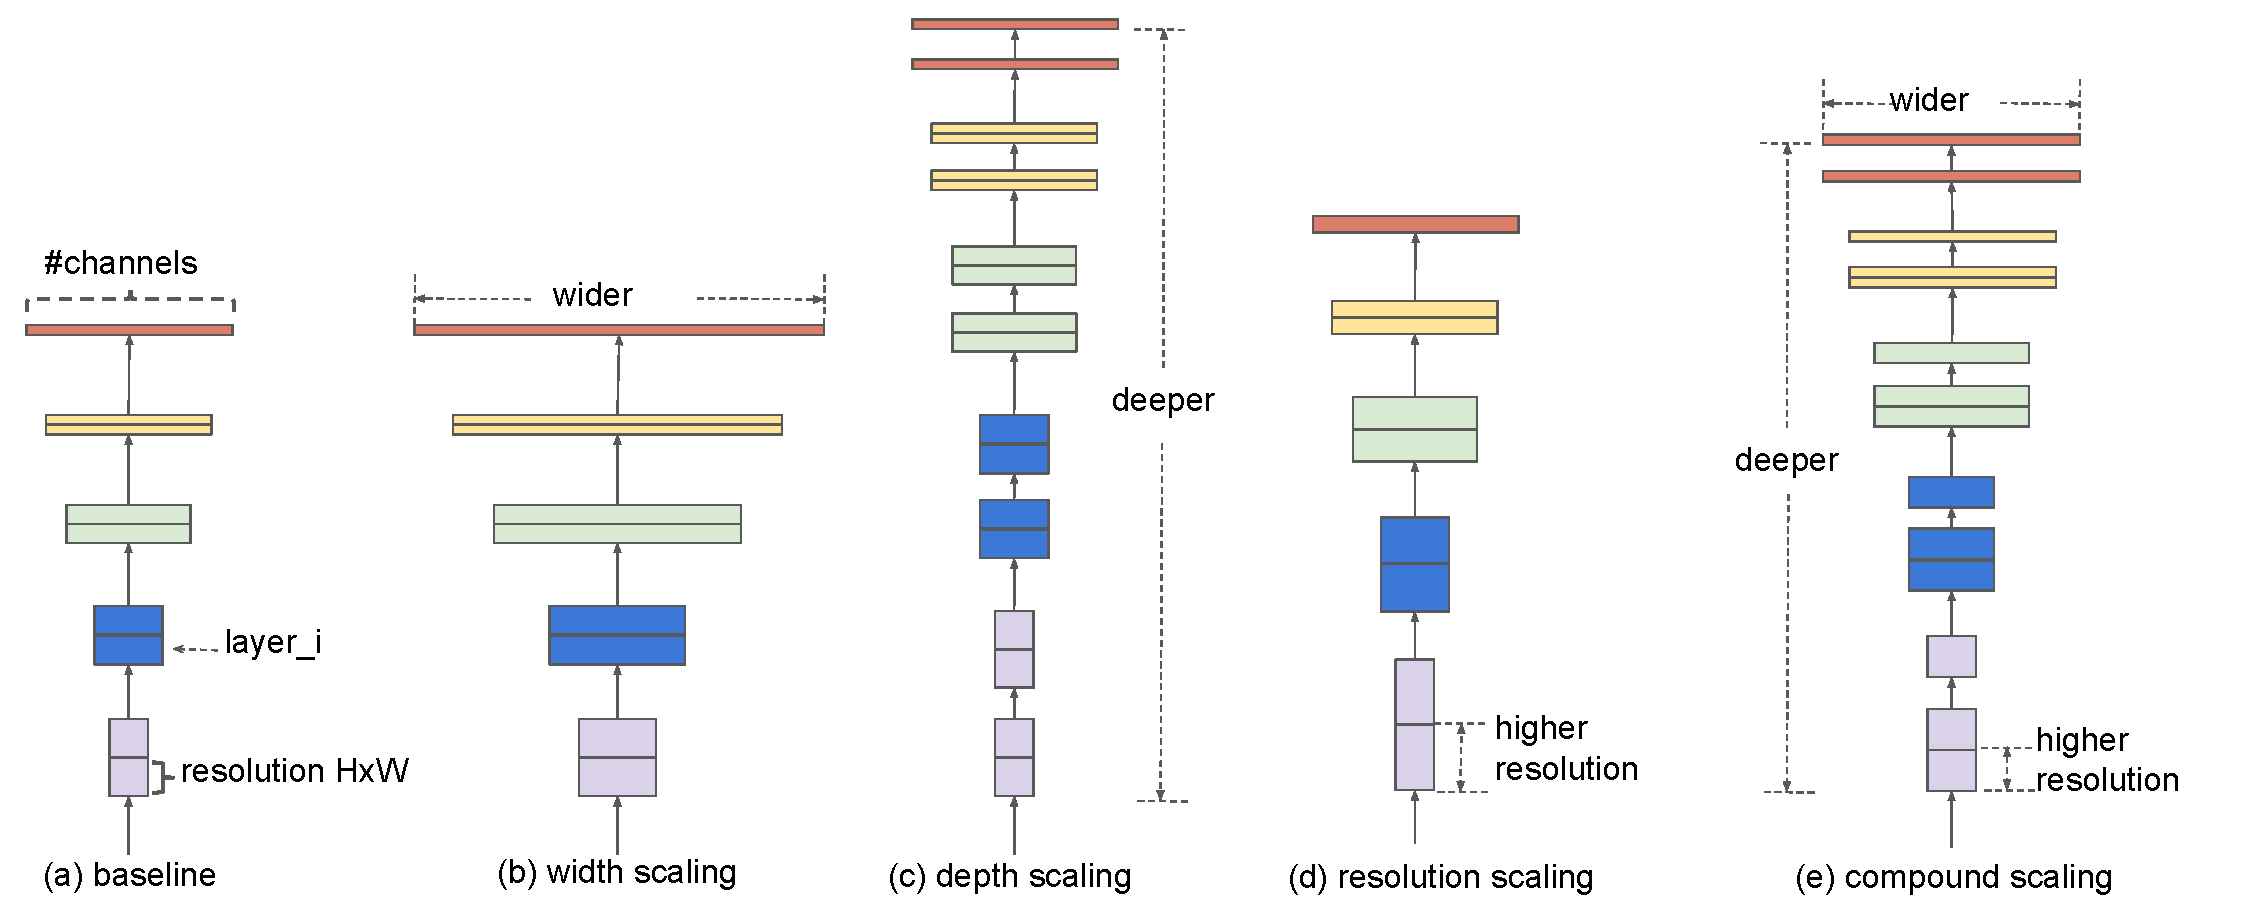
\includegraphics[width=1\linewidth]{Imagenes/scalecompare.pdf}
  \caption{Número de parámetros de la red y precisión en ImageNet.}
  \label{fig:param-precision}
\end{figure}


Tras trabajar este escalado, buscando un óptimo, la red resultante consigue muy buenos resultados para el conjunto de imágenes ImageNet, superando a las otras redes con las que se ha comparado utilizando muchos menos parámetros:

\begin{figure}[H]
  \centering
  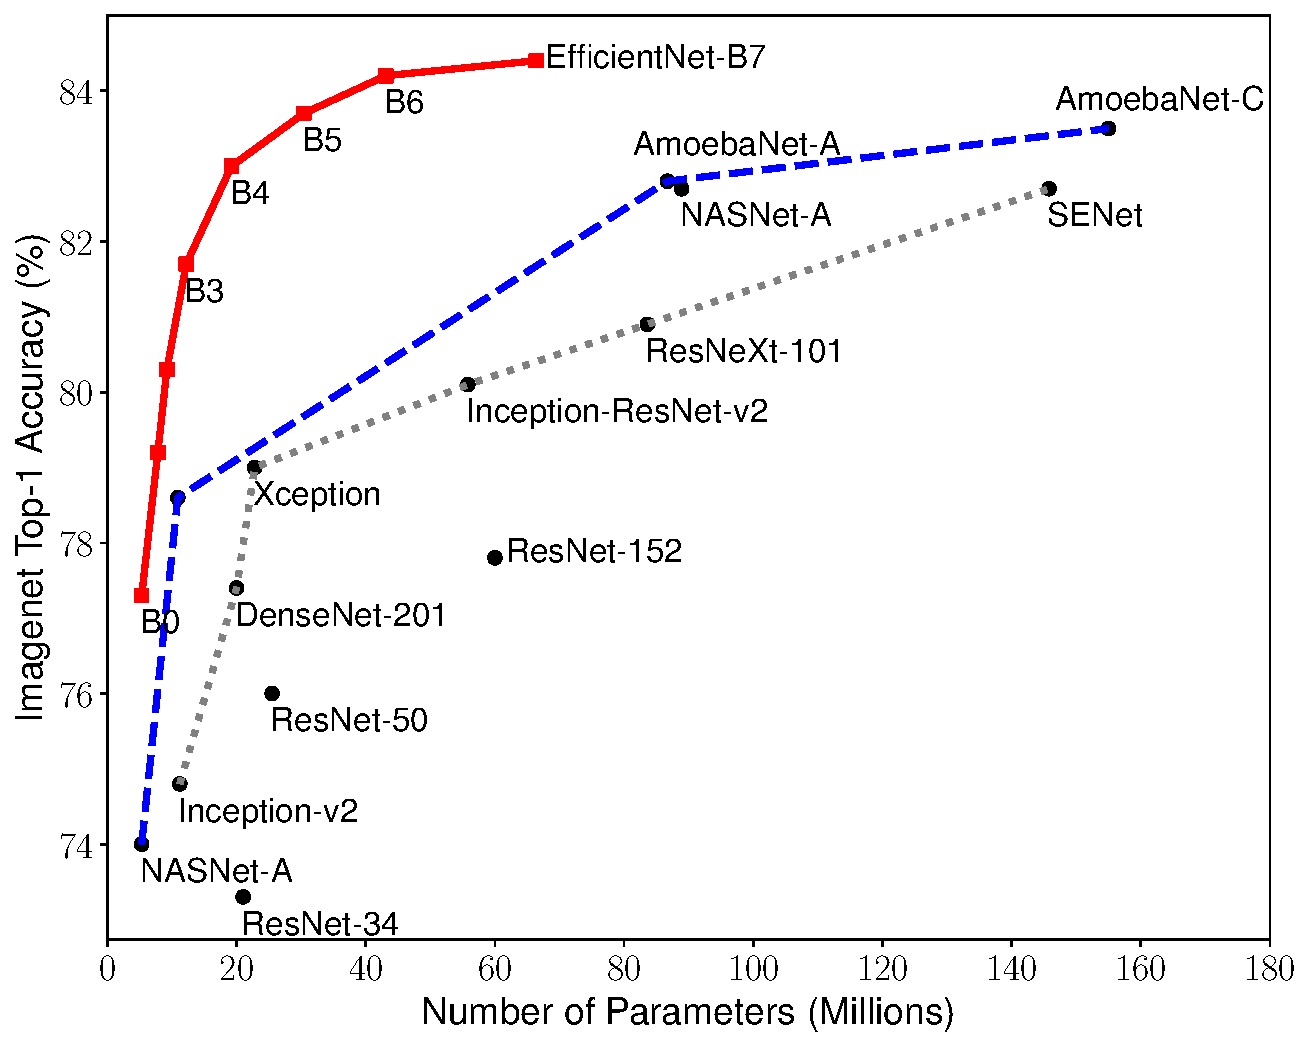
\includegraphics[width=0.5\linewidth]{Imagenes/params.pdf}
  \caption{Número de parámetros de la red y precisión en ImageNet.}
  \label{fig:param-precision}
\end{figure}

Y por último, una vez comprobado que el resultado de ajustar el escalado de la red en el trabajo se trata el problema de la transferencia del conocimiento.

\begin{figure}[H]
  \centering
  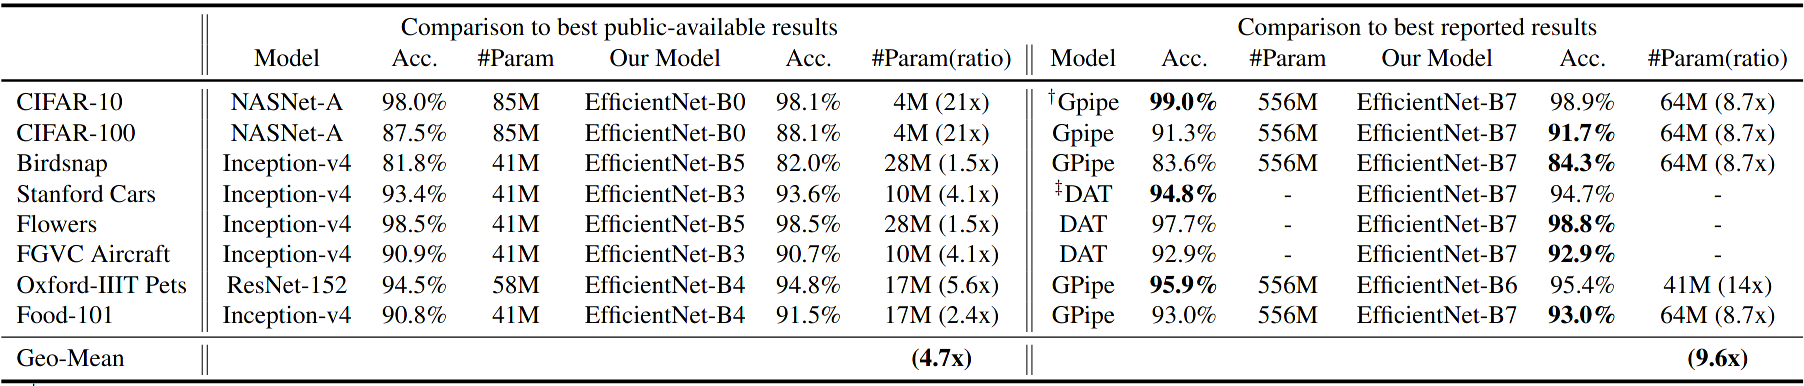
\includegraphics[width=1\linewidth]{Imagenes/cmp-efficient.png}
  \caption{Comparación de EfficientNet con otras redes utilizando múltiples conjuntos de imágenes.}
  \label{fig:param-precision}
\end{figure}

Como resultado, está red con casi diez veces menos parámetros sigue siendo competetitiva, e incluso mejor, que otras redes neuronales, también a la hora de transferir conocimiento a nuevas bases de datos para las que no está entrenada, entre ellas \textbf{Foof101} en la que se obtiene muy buenos resultados. Esto nos demuestra que, si se realiza de forma correcta, la transferencia de conocimiento se puede realizar en cualquier situación y será una parte importante del proyecto, además de que es posible realizar una disminución considerable del número de parámetros de cara a mejorar en tiempo la red.


\newpage

En Otoño de 2019 la Universidad de Stanford presentó un paper llamado \textit{Food Image Classification with Convolutional Neural Networks}. Los autores del mismo tenían la intención de ayudar a los servicios de restauración implementando un sistema que consiga clasificar bien los platos de sus menús para que los clientes tengan una mejor facilidad de elegir. Para ello usarán pesos preentrenados y aplicarán la técnica de transferencia de aprendizaje.

\vspace{3 mm}

En este paper han usado 101000 imágenes del dataset \textbf{Food-101}, dividiéndolas a su vez en el set de entrenamiento y de test. Los pesos preentrenados que se han cogido son los del dataset \textbf{ImageNet}.

\vspace{3 mm}

Las imágenes han sido redimensionadas a un tamaño concreto antes de realizar el entrenamiento, a parte de aplicarles la función de preprocesado del modelo que se esté usando. También se ha usado \textbf{DataAugmentation} para evitar el overfitting.

\vspace{3 mm}

A la hora de realizar la transferencia de aprendizaje se han usado los modelos \textbf{AlexNet}, \textbf{VGG16}, \textbf{ResNet50} y \textbf{InceptionV3}. Al cargar los modelos se ha cambiado la última capa por otra Fully-Connected que tenga tantas neuronas como clases tenga el dataset \textbf{Food-101}. Además de todo esto, por cada modelo se han tuneado las características de las capas superiores, adición de capas Dropout y estimación de los hiperparámetros del optimizador.

\vspace{3 mm}

Para evaluar todos estos modelos se ha usado una top-1 y una top-5 accuracy. La función de pérdida usada es \textbf{categorical cross entropy}. La tabla de resultados de cada una de los modelos es la siguiente:

\vspace{5 mm}

\begin{figure}[H]
  \centering
  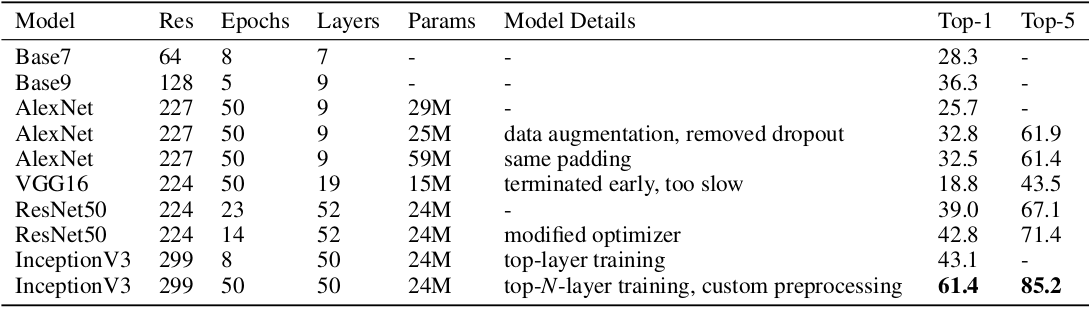
\includegraphics[width=1\linewidth]{Imagenes/tablapaper3.png}
  \caption{Accuracy de Testing}
  \label{fig:sub-first}
\end{figure}

\vspace{5 mm}

Vemos que el modelo que mejores resultados ha proporcionado es \textbf{InceptionV3} con un preprocesado concreto y descongelando un conjunto concreto de capas en el tope de la red. Estos resultados también los tendremos muy en cuenta a la hora de realizar nuestro proyecto ya que se trata de algo similar a lo que tenemos que realizar.


\newpage

Por último nos encontramos con un artículo de la Universidad de Malasia, publicado a principios de este cuatrimestre hace tan solo cinco meses,
\textit{Food Recognition with ResNet-50}\cite{food-resnet}.

Este documento es el que más se centra en el desarrollo del problema como tal, y explica paso a paso el desarrollo del problema, de nuevo haciendo un ajuste fino debido al coste computacional, pero realizando lo que buscamos en nuestro caso.

Explica que en este caso simplemente se aplica un preprocesado de cara a redimensionar las imágenes, de forma que estas tengan la forma de la entrada de la red ResNet-50.

Tras esto explica los fundamentos teóricos ya vistos en teoría y explicados del funcionamiento de la red, desde la forma de trabajar e importancia de cada capa en concreto a la red en conjunto.

Tras explicar la metodología se experimenta con tres bases de datos distintas, \textbf{ETHZ FOOD-101}, \textbf{UECFOOD100} y \textbf{UECFOOD256}. En este caso son imágenes que contienen gran variedad de comida y se han usado los siguientes parámetros para su ajuste fino:

\begin{figure}[H]
  \centering
  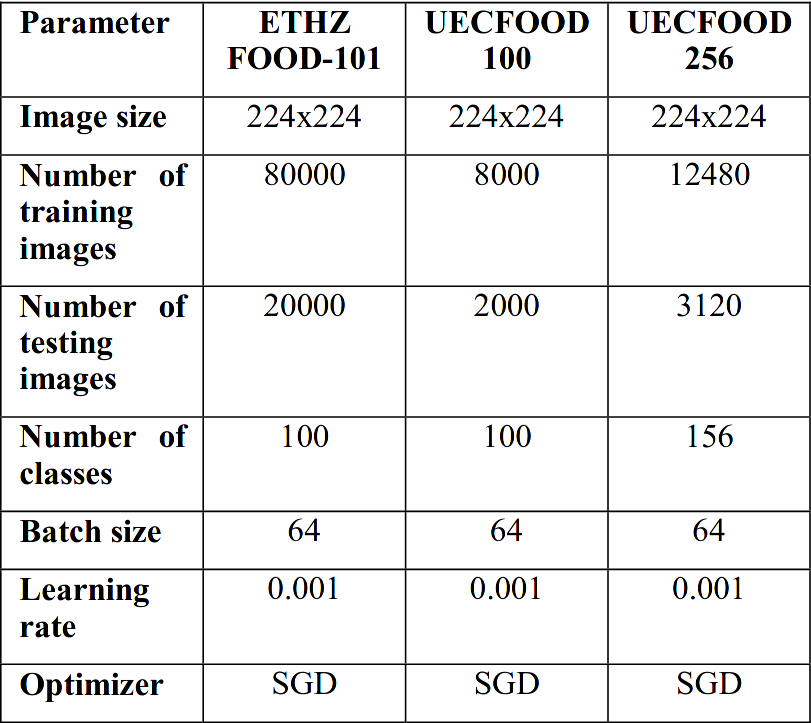
\includegraphics[width=0.5\linewidth]{Imagenes/parametros_food_resnet.png}
  \caption{Parámetros para el ajuste fino de la red con los distintos datasets.}
  \label{fig:sub-first}
\end{figure}

Tras realizar el ajuste fino se comparó con otros modelos y se obtuvieron los siguientes resultados:

\begin{figure}[H]
  \centering
  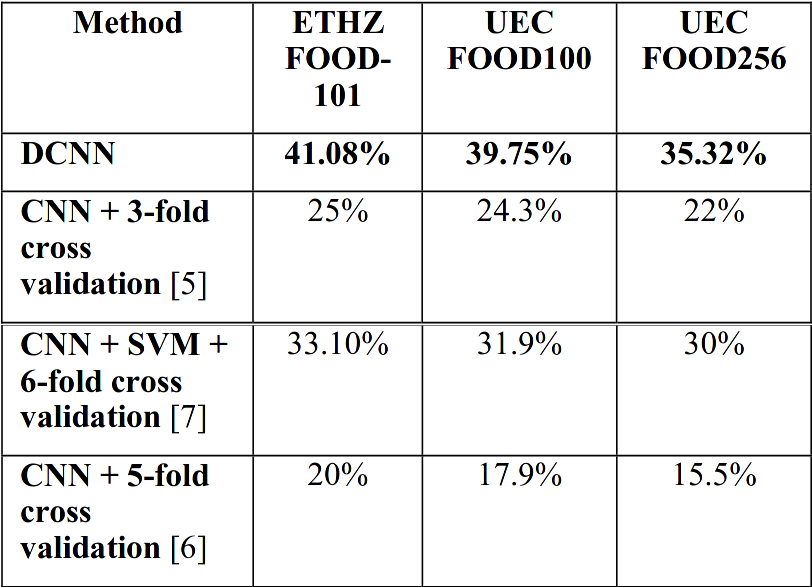
\includegraphics[width=0.5\linewidth]{Imagenes/resultados_resnet_food.png}
  \caption{Resultados y comparación con otros modelos.}
  \label{fig:sub-first}
\end{figure}

Como vemos, se mejora bastante los resultados, pero siguen sin ser unos resultados muy buenos, lo que nos hace pensar que es posible realizar ese ajuste fino, pero si añadimos detalles de metodología vistos en la bibliografía comentada, como por ejemplo el escalado de la red o desconjelando partes del modelo para que también se reentrenen además del ajuste fino de las últimas capas seremos capaces de mejorar el resultado.
